\documentclass[12pt]{article}
\usepackage[utf8]{inputenc}
\usepackage{indentfirst}
\usepackage{graphicx}
\usepackage{hyperref}
\hypersetup{
    colorlinks,
    citecolor=black,
    filecolor=black,
    linkcolor=red,
    urlcolor=blue,
}
\usepackage{tabularx}

\title{\textbf{Intermediate Statistics Report} \\ MOOC Completion through Learner Types}
\author{Octave Cinquanta}
\date{January 2022}

\begin{document}

\maketitle

\section{Abstract}

During the course of Intermediate Statistics, the focus of our work was the analysis of data on a specific Massive Open Online Course. This data included all the results tied to the course itself, such as the videos watched and quizzes completed, and personal information on the participants, such as their gender, country of origin and such. In terms of methods, we used various statistical tests such as the t-test and the ANOVA, and various graphical representations such as mosaic plots and survival charts. We obtained through this analysis the result that the course's completion is significantly dependent on the learner's personal background and his learning habits.

\tableofcontents
\listoffigures
\listoftables

\section{Introduction}

Looking through the data available to us, we noticed that only about 10\% of learners actually completed the whole course. That value is surprisingly low, as since the learners are people who registered themselves to study this course, as such it would be expected that they would want to study it through to the end. Why did only a tenth of the participants actually complete the course ? To try and find an answer to that question, we used several statistical methods to analyse the data, such as correlation tests between variables for instance. Our hypotheses were that the completion of the course was dependent on the learner's personal background, such as their gender, country of origin and socioeconomic status, as well as their own behavior towards the course. Those hypotheses were tested using the methods presented below.

\section{Methods}

This data was provided to us by the FUN MOOC website in order for us to use it as learning material. As such, it can be considered reliable when it comes to this specific course. We focused our analysis on the completion of the course, which we emulated by looking at the number and percentage of videos watched, quizzes completed and certificate obtained. We compared this data with personal information on the learners, such as their gender, the HDI of their origin country and their socioeconomic status. We also looked at and classified the different behaviors of the learners. \\
We used several statistical correlation tests such as the t-test, the ANOVA and the chi test, as well as mosaic plots and survival plots. All of it was done using RStudio with R version 4.0.5 and the following libraries : plyr, dplyr, ggplot2, bbplot, ggrepel, forcats, scales, xtable, MASS, caret, leaps, klaR, graphics, questionr, finalfit, moonBook, survival, ranger, ggfortify and survminer.

\section{Describing the behavior of the learners}

Our objective for this first work on the data-set was to study the proportion of the different types of learners we could identify using given characteristics. The various types of learner behaviors are as such:
\begin{itemize}
    \item The Completer - a learner who has obtained the certificate of completion of the course
    \item The Disengaging Learner - a learner who has answered at least one quiz or submitted at least one assignment but hasn't obtained the certificate
    \item The Auditing Learner - a learner who hasn't answered a single quiz or submitted a single assignment but has watched at least 10\% of the available videos
    \item The Bystander - a learner who hasn't answered a single quiz or submitted a single assignment and who has watched less than 10\% of the available videos
\end{itemize}

\begin{figure}[h]
    \centering
    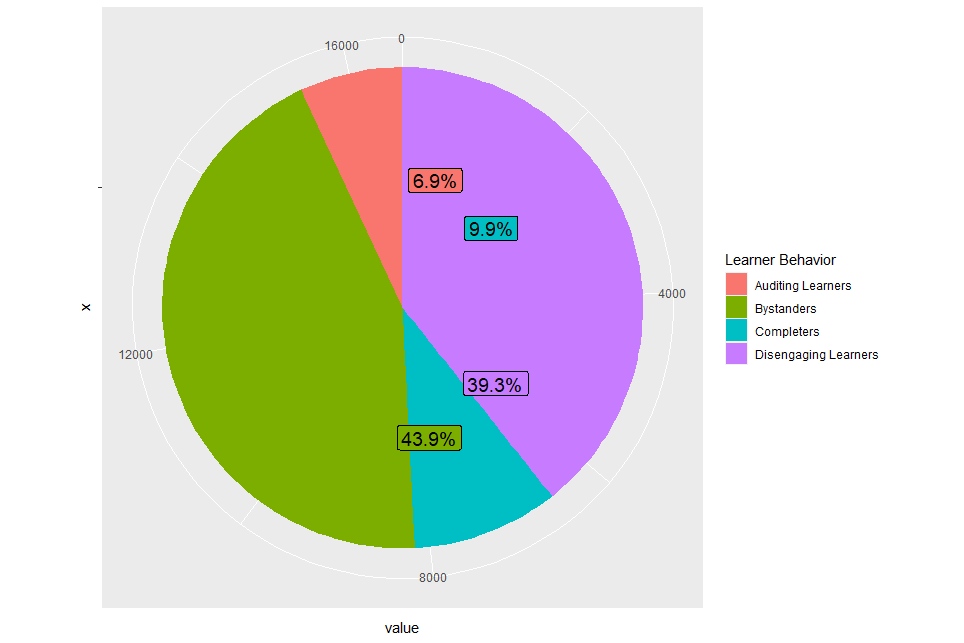
\includegraphics[width=\textwidth]{pie.png}
    \caption{Proportion of each type of learner behavior}
    \label{pie}
\end{figure}

Using a number of filters, we separated the data-set into 4 subsets corresponding to the 4 types of behaviors, counted the number of learner in each category and created a \hyperref[pie]{pie chart} out of those observations. We can see that a slight majority of learners are bystanders, with a proportion of 43.9\% for a total of 7279 learners. The rest of the learners are mainly disengaging learners, with a proportion of 39.3\% for a total of 6527 learners. The two leftover minorities are the completers with a proportion of 9.9\% for a total of 1635 learners and the auditing learners with a proportion of 6.9\% for a total of 1153 learners. \\
What we can deduce from this graph is that there is a majority of people who either enlisted to the course and actually didn't go through with it or gave up extremely quickly because it was either optional, too difficult to approach or simply didn't fit the learner's needs. Most of the remaining learners ended up giving up after a bit of work was put into it, which could have been caused by the difficulty of the course, among many other reasons. A few of the learners actually put the effort necessary to pass the course, and another bunch simply watched the videos, as it may have been their preferred way to learn, and they didn't want to bother with assignments and things of the sort.

\section{Linear Model}
\subsection{T-Test and ANOVAs}

We were tasked for this second part with analyzing the number of videos watched and use various tests to look for correlations between the number of videos and other variables such as the gender, the country of origin's HDI and the  socioeconomic status. First, we started by conducting a t-test with videos and gender. The results are as follows:

\begin{table}[ht]
\centering
\begin{tabular}{rrrrr}
  \hline
 & Estimate & Std. Error & t value & Pr($>$$|$t$|$) \\ 
  \hline
(Intercept) & 16.4672 & 0.1725 & 95.48 & 0.0000 \\ 
  Gender: woman & 0.9664 & 0.3003 & 3.22 & 0.0013 \\ 
   \hline
\end{tabular}
\caption{t-test of videos and gender}
\end{table}

We can see here that the mean value of the number of videos watched by men is 16.4672 videos and by women is 17.4336 (16.4672+0.9664) videos. The p-value we obtained is 0.0013, which is smaller than 0.05, meaning that there is a significant correlation between the gender of the learners and the number of videos they have watched. \\
Secondly, we conducted another type of test, this time an ANOVA, in order to seek a correlation between the country of origin's HDI and the number of videos watched. The results are as follows:

\begin{table}[ht]
\centering
\begin{tabular}{lrrrrr}
  \hline
 & Df & Sum Sq & Mean Sq & F value & Pr($>$F) \\ 
  \hline
Country HDI & 2 & 83050.72 & 41525.36 & 246.54 & 0.0000 \\ 
  Residuals       & 8776 & 1478160.32 & 168.43 &  &  \\ 
   \hline
\end{tabular}
\caption{ANOVA of videos and country HDI}
\end{table}

We can see that this ANOVA gives us a p-value inferior to 0.0001, which is itself inferior to 0.05, meaning that there is a significant correlation between the country of origin's HDI and the number of videos watched. Lastly, we decided to conduct another ANOVA, this time with the gender, country of origin's HDI and socioeconomic status. The results are as follows:

\begin{table}[ht]
\centering
\begin{tabular}{lrrrrr}
  \hline
 & Df & Sum Sq & Mean Sq & F value & Pr($>$F) \\ 
  \hline
Gender & 1 & 1669.10 & 1669.10 & 9.96 & 0.0016 \\ 
  Country HDI & 2 & 80867.52 & 40433.76 & 241.31 & 0.0000 \\ 
  CSP & 10 & 8466.68 & 846.67 & 5.05 & 0.0000 \\ 
  Residuals & 8730 & 1462817.05 & 167.56 &  &  \\ 
   \hline
\end{tabular}
\caption{ANOVA of videos, gender, country HDI and socioeconomic status}
\end{table}

This ANOVA gives us one different p-value for each variable we are studying. The p-values for both gender and country of origin's HDI have already been studied above. The p-value for the socioeconomic status is also inferior to 0.0001, which is itself inferior to 0.05, meaning that there is a significant correlation between the socioeconomic status and the number of videos watched.

\subsection{Model refinement and pairwise comparisons}

We introduced an interaction parameter, namely Gender * Country HDI, in the model we used above, and obtained the following ANOVA table.

\begin{table}[ht]
\centering
\begin{tabular}{lrrrrr}
  \hline
 & Df & Sum Sq & Mean Sq & F value & Pr($>$F) \\ 
  \hline
Gender & 1 & 1669.10 & 1669.10 & 9.96 & 0.0016 \\ 
  Country\_HDI.fin & 2 & 80867.52 & 40433.76 & 241.32 & 0.0000 \\ 
  CSP & 10 & 8466.68 & 846.67 & 5.05 & 0.0000 \\ 
  Gender:Country\_HDI.fin & 2 & 435.25 & 217.63 & 1.30 & 0.2729 \\ 
  Residuals & 8728 & 1462381.80 & 167.55 &  &  \\ 
   \hline
\end{tabular}
\caption{ANOVA with a newly-introduced interaction parameter}
\end{table}

As we can see, we obtained multiple p-values under 0.05, meaning that all three of the variables Gender, Country HDI and Socioeconomic Status have a significant impact on the number of videos watched by the learners. However, our introduced interaction parameter has a p-value larger than 0.05, meaning that there is no significant correlation between the gender of the learners and their origin country's HDI. We can also have a look at the obtained F-values, which are an indication of a difference in the groups' means. The country HDI has a large F-value, indicating important differences in its groups' means, while the other two variables and the interaction parameter' F-values are relatively small, indicating an absence of major differences in their groups' means, and that is especially true for the interaction parameter. \\

We conducted three chi-tests using these variables and obtained the following results:
\begin{itemize}
    \item Gender and Country HDI, p-value $<$ 2.2e-16
    \item Gender and Socioeconomic Status, p-value = 2.225e-11
    \item Socioeconomic Status and Country HDI, p-value $<$ 2.2e-16
\end{itemize}
All obtained p-values are below 0.05, meaning that we can infer that there is a relationship between all three variables. \\

\begin{figure}[h]
    \centering
    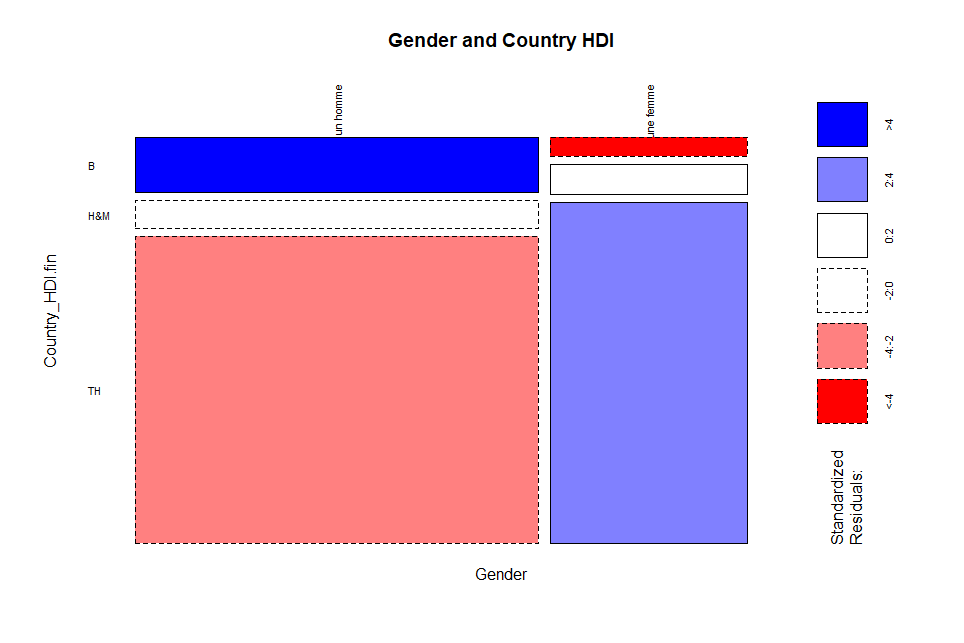
\includegraphics[width=\textwidth]{mosaic.png}
    \caption{Mosaic plot of the Gender and Country HDI variables}
    \label{mosaic}
\end{figure}

The mosaic plot we obtained tells us that there is more data on men than there is on women. The plot also indicates a significant over-representation of men in countries with poor HDI, and a significant under-representation of women in those countries. Likewise, we see that for countries with a high HDI, there is an over-representation of women and an under-representation of men. \\

We used Tukey HSD to have a look at the pairwise differences between learners of different socioeconomic status.

\section{Logistic Regression}

\subsection{Producing an Odd-Ratios table}

\begin{table}[ht]
\centering
\begin{tabular}{rrrrrr}
  \hline
 & OR & 2.5 \% & 97.5 \% & p & \\ 
  \hline
(Intercept) & 0.15 & 0.12 & 0.18 & 0.00 & ***\\ 
  Genderune femme & 1.13 & 1.00 & 1.27 & 0.04 & *\\ 
  Country\_HDI.finH\&M & 1.24 & 0.93 & 1.64 & 0.14 & \\ 
  Country\_HDI.finTH & 1.49 & 1.23 & 1.82 & 0.00 & ***\\ 
   \hline
\end{tabular}
\caption{Odd-Ratios Table of gender and country HDI}
\end{table}

We used a logistical regression model to obtain the above Odd-Ratios table. The parameters observed are whether the learners have passed the exam in function to their gender and their country of origin's HDI. As we can see with the obtained p values, the gender has a small impact on the success of the learners, but the country of origin's HDI when it is a very high HDI has a very significant impact on whether the learner passes the exam or not.

\subsection{Poisson models for count data}

\begin{figure}[h]
    \centering
    
\includegraphics[width=\textwidth]{plot.png}
    \caption{Quantile Quantile Plot of the videos viewed}
    \label{mosaic}
\end{figure}

We plotted a QQ Plot of the videos viewed variable and we can observe that the residuals do not follow a normal distribution, complicating the analysis of the data.

\section{Survival Analysis}

We decided to create a survival plot of our dataset, focusing on the type of learners, especially disengaging learners and auditing learners, since completers would not be able to drop out of the course and bystanders would not survive the course at all. The obtained results show us that the auditing learners almost all drop out quite fast, while the disengaging learners steadily lose grip of the course over time.

\begin{figure}[h]
    \centering
    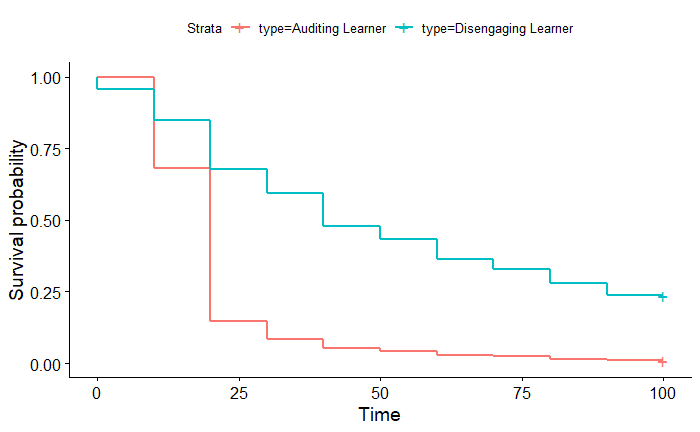
\includegraphics[width=\textwidth]{surv.png}
    \caption{Survival of the Disengaging Learners and the Auditing Learners}
    \label{mosaic}
\end{figure}

\newpage
\section{Discussion}

Throughout the use of several statistical tests, we were able to determine the impact of various personal details on one's learning experience. We found correlations between the gender, the HDI of the country of origin and the socioeconomic status and we obtained the following. We saw that women have a tendency to watch slightly more videos than men, and as such complete more of the course in general, however, we saw that this impact on the completion is quite small and barely significant. We also saw that the country of origin's HDI had a rather significant impact on the course completion, mostly that the country of origin having a high HDI had a very significant impact on the completion while the country having a medium HDI does not impact the completion whatsoever. We also saw that the socioeconomic status was relevant when it comes to the completion. \\
We also analysed the behaviors of the learners, and found out that most of the learners either do not participate in the course at all, or end up giving up slowly through time. The rest either completes the course entirely or somehow stops not at the beginning but still very prematurely. 

\end{document}